In this task we were to design and implement a real time system. The task is self-chosen.
\subsection{Traffic light}
We chose to design and implement a traffic light control system. These kind of systems are subject to real time requirements.\\
A basic model of the system can be seen in figure~\ref{fig:traffic_light}. It model as a road that has a primary road (the horisontal) and a secondary (the vertical). The primary road must be in the passable or ``green'' state as much as possible. This state is called the primary state.\\
When a car wants to cross the primary road, the light must change within a maximum amount of time. However, it sould not be possible for the secondary road to gain precedence over the primary road, if there are heavy traffic on the primary road.\\
We therefore set the following rules:
\begin{enumerate}
 \item When there are cars on the primary road, the lights cannot change to secondary state
 \item When there are no cars on the primary road, the lights can change to secondary state
 \item The light cannot be in the primary state for an unlimited amount of time
\end{enumerate}

\begin{figure}
\centering
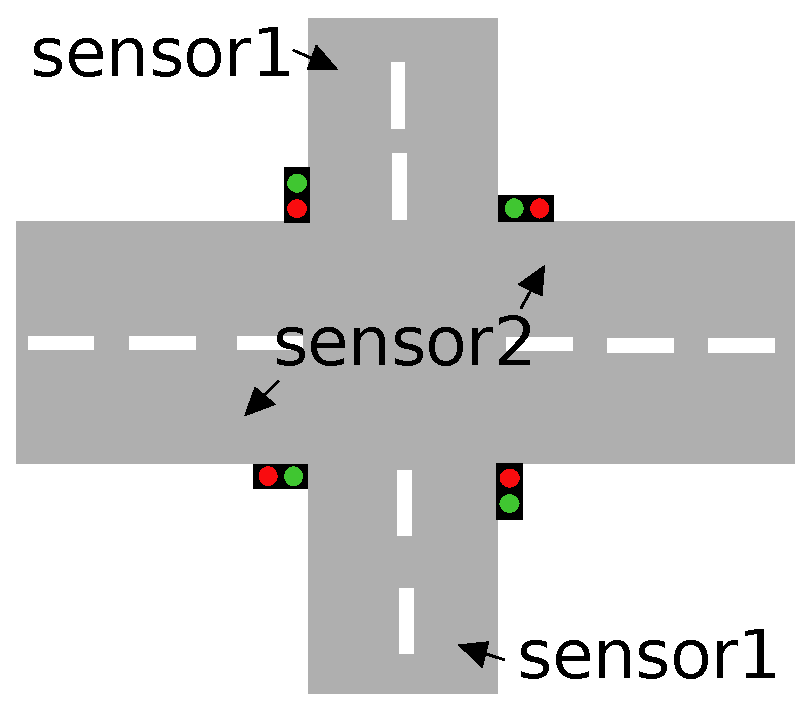
\epsfig{file=fig/Traffic_Light.eps, height=2in}
\caption{Basic model of traffic light system}
\label{fig:traffic_light}

\end{figure}

\subsection{design}
The traffic light control system has the following logic visually depicted in figure~\ref{fig:traffic_light_design}; Transition 1 only occurs if there is a no sensor input from sensor2 or the timeout has occured \emph{and} sensor1 is triggered.\\
Transition 2 occurs automatically after a timeout.

\begin{figure}
\centering
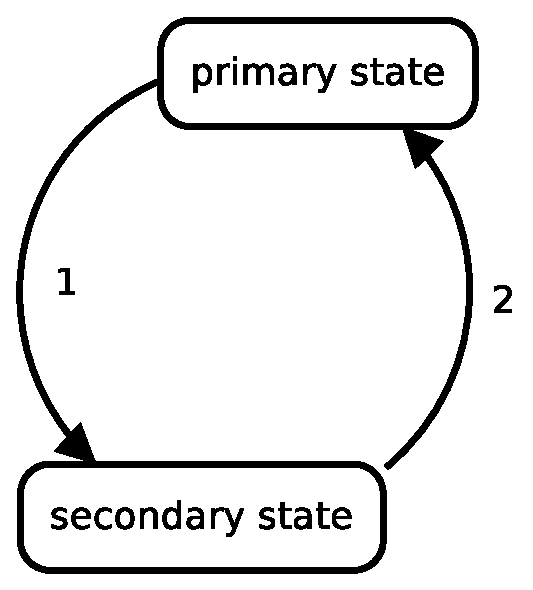
\epsfig{file=fig/Traffic_Light_Design.eps, height=2in}
\caption{States of traffic light system}
\label{fig:traffic_light_design}
\end{figure}
The real time requirements of this specification kind of resembles a sporadic scheduler, with the primary road having the highest priority, but only within a period, and then drops below the secondary roads priority. The budget is then relinquished when a change state cycle has occurred.
\subsection{Implementation}
The system consists of two processes; one process runs the sensor input part, the other does the light change. The two processes communicate via IPC (see section~\ref{sec:ipc}).\\
The light control process does most of the logic. The light state is protected with a mutex (acutally a binary semaphore), and uses three (acutally four, counting main) threads. One for recieving IPC, as this is a blocking call. One for taking care of the release policy asynchronous and one for taking care of the light switch. This thread tries to keep the mutex for itself for as long as possible. The policy thread can decide if the timer thread must give up the mutex based on the input from the IPC thread and from a ``random car generator'' used for testing.

\subsection{Test}
The test was done using visual inspection, using the graphical user interface and the debug output. The system behaved as expected, and did not change to the secondary state if cars were still arriving, but did switch if the timeout was reached or cars did not arrive.